\documentclass[12pt,a4paper]{article}
\usepackage{pgf}
\usepackage{svg}
\usepackage{gensymb}
\usepackage[french]{babel}
\usepackage{forest}
\usepackage{tikz}
\usepackage{stanli}
\usepackage{xcolor}
\usepackage{afterpage}
\usepackage{soul}
\usepackage{listings}
\usepackage{multirow}
\usepackage{subfig}
\usepackage{svg}
\usepackage{rotating}
\usepackage{siunitx}
\usepackage[a4paper,top=2cm,bottom=1.5cm,left=1.5cm,right=1.5cm,marginparwidth=1.75cm]{geometry}

\usepackage{amsmath}
\usepackage{graphicx}
\usepackage[colorlinks=true, allcolors=blue]{hyperref}

\newcommand{\blue}[1]{\textcolor{blue}{#1}}
\newcommand{\red}[1]{\textcolor{red}{#1}}

\title{}
\author{}
\date{}

\begin{document}
	
	\newcommand{\subf}[2]{%
		{\small\begin{tabular}[t]{@{}c@{}}
				#1\\#2
		\end{tabular}}%
	}
	
	\begin{titlepage}
		\begin{center}
			\vspace*{3cm}
			
			\Huge
			\textbf{M1 C++}
			
			\vspace{0.3cm}
			\Huge
			Simulation numérique d'un dispositif de refroidissement
			
			\vspace{0.8cm}
			\large
			
			
			
			\vspace{0.5cm}
			\LARGE
			
			
			\vspace{1.5cm}
			
			\textbf{}
            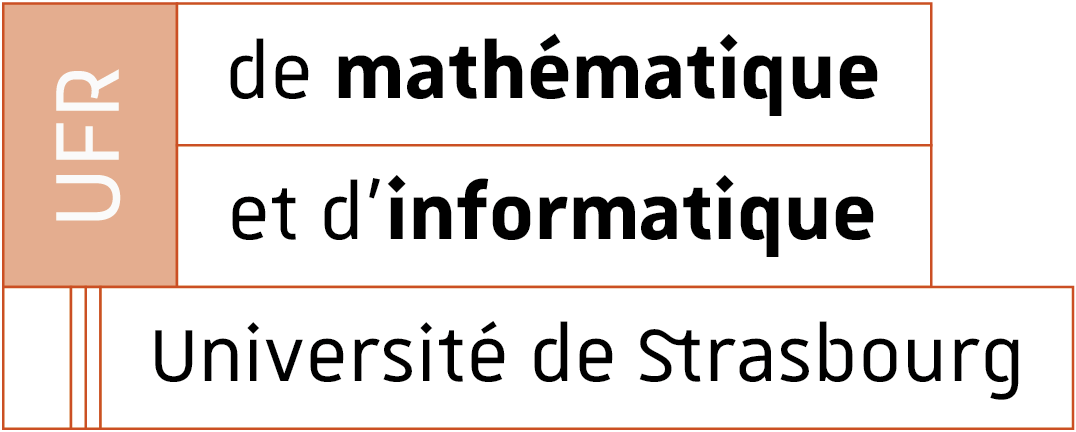
\includegraphics[width=0.4\textwidth]{logo_ufr.png}
			
			\vfill
			
			
			
			\vspace{0.8cm}
			
			
			
			\Large
			
			
			
			
		\end{center}
		\Large
		\begin{tabbing}
			\hspace*{1em}\= \hspace*{8em} \= \kill % set the tabbings
			\> Nom:\>  Carpi Lapi \\
			\> Prénom:\>  Giulio \\
			\> Master:\>  CSMI  \\
			\> Année:  \> 2023 \\
			\> Attribué : \> 25 octobre 2023\\
			\> Dû: \>  15 décembre 2023
		\end{tabbing}
		
	\end{titlepage}
	
	
	\tableofcontents
	\section{Introduction}

	Ce projet a pour but de réaliser un programme C++ permettant d'étudier le comportement
	thermique d'un dispositif de refroidissement d'un micro-processeur. Un des moyens généralement
	utilisé pour réguler la température d'un processeur est l'utilisation d'un ventilateur. Le soufflage
	d'air va permettre d'évacuer la chaleur par convection sur la surface du processeur. Pour améliorer
	ce processus, le processeur est généralement attaché à un dissipateur (composé de plusieurs ailettes)
	qui est un élement très conducteur de chaleur. Ce disposif supplémentaire,
	permet d'augmenter la surface d'échange avec le flux d'air et d'ainsi refroidir plus efficacement
	le composant électronique.\\
	
	Pour ce projet, nous allons nous intéresser uniquememt à la simulation thermique d'une seule ailette du dissipateur.
	Les données du problème sont : la géométrie de l'ailette, qui est décrite par les longueurs $L_x$ , $L_y$ et $L_z$,
	le flux de chaleur $\Phi_p$ généré par le processeur et la température ambiante $T_e$. De plus, nous supposons que l'ailette est suffisamment
	mince pour considérer le problème unidimensionnel. La température $T$ en un point donné dépendra uniquement de sa position selon $x$ et de l'instant $t$.\\

	En prenant en compte les pertes latérales par convection avec l'air, l'équation de la chaleur dans une ailette 
	définie sur le domaine $x = [0, L_x]$ est donnée par :\\

	$$\rho C_p \frac{\partial T}{\partial t} - k \frac{\partial^2 T}{\partial x^2} + \frac{h_c p}{S} (T - T_e) = 0$$\\

	avec $\rho$ la densité, $C_p$ la chaleur spécifique à pression constante, $k$ la conductivité thermique, $h_c$ le coefficent 
	de transfert de chaleur surfacique, $S = L_yL_z$ l'aire d'une section transversale et $p = 2(L_y + L_z)$ le périmètre d'une section transversale. 
	Au niveau des conditions aux limites, nous supposons connaître le flux de chaleur $\Phi_p$ dégagé par le processeur en $x = 0$ et 
	nous faisons l'hyphothèse que le transfert de chaleur en $x = L_x$ est négligeable par rapport au flux apporté sur la section longitudinale. 
	Cette modélisation nous conduit finalement à la recherche de la température $T$ définie sur le domaine $x = [0, L_x]$ qui vérifie :

	$$\rho C_p \frac{\partial T}{\partial t} - k \frac{\partial^2 T}{\partial x^2} + \frac{h_c p}{S} (T - T_e) = 0$$
	$$-k \frac{\partial T}{\partial x} \bigg|_{x=0} = \Phi_p$$
	$$ -k \frac{\partial T}{\partial x} \bigg|_{x=L_x} = 0$$

	Les valeurs des paramètres utilisés pour les simulations sont données dans la table 1.
	On a choisi les propriétés physiques en considérant que l'ailette est constituée d'un alliage d'aluminium. \\

	\begin{table}[h]
		\centering
		\begin{tabular}{|c|c|c|}
			\hline
			Nom & Valeur & Unité \\
			\hline
			$\rho$ & 2700 & \si{kg/m^3} \\
			\hline
			$C_p$ & 940 & \si{J/(kg\cdot K)} \\
			\hline
			$k$ & 164 & \si{W/(m\cdot K)} \\
			\hline
			$T_e$ & 20 & $^{\circ}$C \\
			\hline
			$\Phi_p$ & 1.25 $\cdot 10^5$ & W/$m^2$ \\
			\hline
			$h_c$ & 200 & W/($m^2 \cdot K$) \\
			\hline
			$L_x$ & 0.04 & m \\
			\hline
			$L_y$ & 0.004 & m \\
			\hline
			$L_z$ & 0.05 & m \\
			\hline
		\end{tabular}
		\caption{Valeurs des paramètres géométriques et physiques}
		\label{table:exemple}
	  \end{table}

	Cependant, les valeurs des paramètres pourront être modifiées dans le but d'analyser l'impact du paramètre sur le résultat.
	De plus, la valeur du coefficent de transfert de chaleur surfacique $h_c$ est donné dans ce tableau pour le cas où le ventilateur est en marche.
	On pourra également traiter le cas où le ventilateur est éteint en utilisant $h_c = 10 W/(m^2 \cdot K)$. \\

	\subsection{Modèle stationnaire}

	Nous commençons par traiter le cas stationnaire, c'est-à-dire par calculer la distribution de température lorsque le temps t tend vers l'infini.
	On enlevera alors la dérivée en temps présente dans l'équation donnée, qui devient alors :
	
	$$-k \frac{\partial^2 T}{\partial x^2} + \frac{h_c p}{S} (T - T_e) = 0$$\\

	Pour résoudre cette EDP, nous allons utiliser la métode des différences finies.
	Pour cela nous décomposons le segment $[0,L_x]$ en $M$ intervalles de longueur $h = L_x/M$.
	Nous obtenons ainsi un maillage composé de $M+1$ points d'abscisses $x_i = i\cdot h, i = 0,...,M$.
	La solution numérique sera alors décrite par ces $M+1$ points et on notera $T_i$ la température calculée au point $x_i$.
	Nous allons ensuite utiliser un développement de Taylor pour approcher la dérivée seconde. Donc pour $i = 1,...,M-1$, nous avons :

	$$T(x_i+h) = T(x_i) + hT'(x_i) + \frac{h^2}{2}T''(x_i) + \frac{h^3}{6}T'''(x_i) + O(h^4)$$
	$$T(x_i-h) = T(x_i) - hT'(x_i) + \frac{h^2}{2}T''(x_i) - \frac{h^3}{6}T'''(x_i) + O(h^4)$$

	Ce qui donne :

	$$T(x_i+h) + T(x_i-h) = 2T(x_i) + h^2T''(x_i)) + O(h^4)$$

	et donc :

	$$ \frac{\partial^2 T}{\partial x^2}(x_i) \approx \frac{T_{i-1} - 2T_i + T_{i+1}}{h^2}$$\\

	Nous obtenons ainsi les équations discrètes du problème définies sur tous les noeuds internes :

	$$ -k\frac{T_{i-1} - 2T_i + T_{i+1}}{h^2} + \frac{h_c p}{S} (T - T_e) = 0, \forall i \in [1,M-1]$$\\

	Reste à appliquer les conditions aux limites pour fermer le système :

	$$-k \frac{\partial T}{\partial x} \bigg|_{x=0} \approx -k\frac{T_1 - T_0}{h} = \Phi_p$$
	$$-k \frac{\partial T}{\partial x} \bigg|_{x=L_x} \approx -k\frac{T_{M-1} - T_M}{h} = 0$$\\

	En combinant toutes ces informations, le problème discret est décrit par la résolution d'un système
	$AX=F$ avec $A$ une matrice tridiagonale (taille $M + 1 \times M + 1$ ), $F$ le vecteur second membre
	(taille $M + 1$) et $X$ le vecteur solution représentant la température en chaque point de discrétisation
	$x_i$ avec $i \in [0,M]$.

	\[
	\underbrace{
	\begin{bmatrix}
		b_{0} & c_{0} & 0 & 0 & \cdots & 0 \\
		a_{1} & b_{1} & c_{1} & 0 & \cdots & 0 \\
		0 & a_{2} & b_{2} & c_{2} & \cdots & 0 \\
		\vdots & \vdots & \vdots & \vdots & \ddots & \vdots \\
		0 & \cdots & \cdots & a_{M-1} & b_{M-1} & c_{M-1} \\
		0 & \cdots & \cdots & 0 & a_{M} & b_{M}
	\end{bmatrix}
	}_{\text{$A$}}
	\underbrace{
	\begin{bmatrix}
		T_{0} \\
		T_{1} \\
		T_{2} \\
		\vdots \\
		T_{M-1} \\
		T_{M}
	\end{bmatrix}
	}_{\text{$X$}}
	=
	\underbrace{
	\begin{bmatrix}
		F_{0} \\
		F_{1} \\
		F_{2} \\
		\vdots \\
		F_{M-1} \\
		F_{M}
	\end{bmatrix}
	}_{\text{$F$}}
\]

Nous allons résoudre ce système grâce à une décompisition LU, or L = "lower triangular matrix" est une matrice triangulaire inférieure et U = "upper triangular matrix" une matrice triangulaire supérieure.
Nous avons :


\[
\mathbf{L} = \begin{bmatrix}
	1 & 0 & 0 & 0 & \cdots & 0 \\
	a^*_{1} & 1 & 0 & 0 & \cdots & 0 \\
	0 & a^*_{2} & 1 & 0 & \cdots & 0 \\
	\vdots & \vdots & \vdots & \ddots & \vdots & 0 \\
	0 & \cdots & 0 & a^*_{M-1} & 1 & 0 \\
	0 & \cdots & \cdots & 0 & a^*_{M} & 1
\end{bmatrix}
\]

\[
\mathbf{U} =\begin{bmatrix}
	b^*_{0} & c_0 & 0 & 0 & \cdots & 0\\
	0 & b^*_{1} & c_1 & 0 & \cdots & 0\\
	\vdots & \vdots & \vdots & \vdots & \ddots & \vdots \\
	0 & \cdots & \cdots & 0 & b^*_{M-1} & c_{M-1}\\
	0 & \cdots & \cdots & \cdots & 0 & b^*_{M}
\end{bmatrix}
\]

\underline{Note Bene} : Je n'ai pas utilisé la même décomposition LU suggérée dans l'énoncé.

	\subsection{Modèle instationnaire}

	\section{Structure du projet}

	\subsection{Compilation}
	Pour compiler l'intégralité du programme depuis le terminal, commencez par créer un répertoire appelé \texttt{build} en utilisant la commande \texttt{mkdir build}.
	À l'intérieur du répertoire \texttt{build}, utilisez la commande \texttt{cmake ..} pour effectuer la configuration de la compilation en se basant sur le fichier \textit{CMakeLists.txt}.
	Enfin, procédez à la compilation du programme en utilisant la commande \texttt{make}.\\

	Vous pouvez paramétrer le modèle en utilisant le fichier de configuration \textit{simu.cfg}.

	\subsection{Structure et contenu des différentes répertoires}

	Voici une arborescence du dossier \textit{projet} :
	\forestset{
  L1/.style={fill=green,},
  L2/.style={fill=orange,edge={orange,line width=2pt}},
  L3/.style={fill=yellow,edge={yellow,line width=2pt}},
  L4/.style={fill=pink,edge={pink,line width=2pt}},
}

\begin{forest}
    for tree={
        grow=0,reversed, % tree direction
        parent anchor=east,child anchor=west, % edge anchors
        edge={line cap=round},outer sep=+1pt, % edge/node connection
        rounded corners,minimum width=15mm,minimum height=8mm, % node shape
        l sep=10mm % level distance
    }
  [\textit{project},L1
    [\textit{include},L2
		[\textit{vector.hpp},L3]
		[\textit{tridiag.hpp},L3]
		[\textit{mesh.hpp},L3]
        [\textit{config.hpp},L3]
		[\textit{solver.hpp},L3]
		[\textit{stationary.hpp},L3]
        [\textit{instationary.hpp},L3]
		[\textit{constantFlux.hpp},L3]
		[\textit{heatFlux.hpp},L3]
    ]
    [\textit{src},L2
		[\textit{vector.cpp},L3]
		[\textit{tridiag.cpp},L3]
		[\textit{mesh.cpp},L3]
		[\textit{config.cpp},L3]
		[\textit{solver.cpp},L3]
		[\textit{stationary.cpp},L3]
		[\textit{instationary.cpp},L3]
		[\textit{constantFlux.cpp},L3]
		[\textit{heatFlux.hpp},L3]
		[\textit{main.cpp},L3]
	]
	[\textit{test},L2]
	[\textit{results},L2]
	[\textit{CMakeLists.txt}]
	[\textit{simu.cfg}]
	[\textit{README.md}]
  ]
\end{forest}

	
Pour mieux traiter ce projet, j'ai décidé de créer une classe \texttt{Tridiag}, définie dans le fichier \textit{tridiag.hpp}, et une classe \texttt{Vector}, définie dans le fichier \textit{vector.hpp}.
La classe \texttt{Config}, définie dans le fichier \textit{config.hpp}, lit le fichier \textit{simu.cfg} et initialise toutes les valeurs des paramètres géométriques et physiques nécessaires à la résolution du problème.
La classe \texttt{Solver}, définie dans le fichier \textit{solver.hpp}, est responsable, avec ses fonctions \textit{BuildLU()}, \textit{Forward()}, et \textit{Back()},
de la résolution du système $AX=B$ en remplissant le \texttt{Vector} \texttt{M\_X}, attribut de la classe, avec les solutions.
Ces 4 classes sont communes aux deux modèles.\\

La class \texttt{Mesh}, définie dans le fichier \textit{mesh.hpp} est responsable de la création du maillage, ainsi que du fichier \textit{mesh.vtk}
qui peut être lu par le logiciel de visualisation \textit{ParaView} qui sert à la visualisation 3D du maillage.\\

Nous avons ensuite les deux classes \texttt{Stationary}, définie dans le fichier \textit{stationary.hpp}, et \texttt{Instationary}, définie dans le fichier \textit{instationary.hpp},
qui sont responsables de la création des deux modèles stationnaire et instationnaire.
Elles utilisent les classes susmentionnées pour leur résolution.

	\subsection{Contenu du répertoire \textit{results}}

	\section{Analyse des résultats}

	\subsection{Solution 1D}

	\subsection{Solution 3D}


	
\end{document}